


%\VignetteIndexEntry{Using icenReg}

\documentclass[a4paper]{article}
%\documentclass[11pt]{book}
\usepackage{amsmath, amsthm}
\usepackage[pdftex]{graphicx}
\usepackage{psfrag,epsf}
\usepackage{enumerate}
\usepackage{natbib}
\usepackage{float}
\restylefloat{table}

\usepackage{amssymb}
\usepackage{multirow}
\usepackage{float}


%\VignetteIndexEntry{icenReg}


\usepackage{Sweave}
\begin{document}

\Sconcordance{concordance:icenReg.tex:icenReg.Rnw:%
1 13 1 1 0 635 1}


\title{Using {\bf{icenReg}} for interval censored data in {\bf{R} } \\ v1.3.5}
\author{Clifford Anderson-Bergman}
\maketitle


\tableofcontents

\section{Introduction}



This manual is meant to provide an introduction to using {\bf icenReg} to analyze interval censored data. It is written with expectation that the reader is familiar with basic survival analysis methods. Familiarity with the Kaplan Meier curves, survival regression models (Cox PH, AFT and proportional odds) and basic Bayesian principles should be sufficient for all that is covered in this text.

\subsection{Interval Censoring}

Interval censoring occurs when a response is known only up to an interval. A classic example is testing for diseases at a doctor's clinic; if a subject tests negative at $t_1$ and positive at $t_2$, all that is known is that the subject acquired the disease in ($t_1$, $t_2$), rather than an exact time. Other classic examples include examining test mice for tumors after sacrifice (results in \emph{current status} or \emph{case I} interval censored data, in which all observations are either left or right censored, as opposed to the more general \emph{case II}, which allows for any interval), customer choice models in economics (customers are presented a price for a product and chose to purchase or not, researcher wants to know distribution of maximum spending amount; this results in current status data again), data reduction methods for sensor analyses (to reduce load on sensor system, message is intentionally surpressed if outcome is in an expected region) and data binning (responses reported only up to an interval, in some cases to keep the subjects anonymous, in some cases to reduce size of data). 

  
Often interval censoring is ignored in analysis. For example, age is usually reported only up to the year, rather than as a continuous variable; when a subject reports that their age is 33, the information we have is really that their age is in the interval [33,34). In the case that these intervals are very short relative to the question of interest, such as with reported age when the scientific quesiton is about age of onset of type II diabetes, the bias introduced by ignoring the interval censoring may besmall enough to be safely ignored. However, in the case that the width of intervals is non-trivial, statistical methods that account for this should be used for reliable analysis. 
  
Standard notation for interval censoring is that each subject has a true event time $t_i$ which is potentially unobserved. Rather, we observe a response interval $l_i,r_i$ such that the true event time is known to have occurred within. Default behavior is to assume this an half open, half closed interval, i.e. $t_i \in (l_i, r_i]$\footnote{In {\bf icenReg}, whether the boundaries of the interval are included or not can be controlled by the option \texttt{B} in the model fitting functions.}. An exception to the rule in this notation is that $(t_i, t_i]$ always implies that event $i$ is uncensored with event time at $t_i$, despite this being an undefined interval. This allows for uncensored observations ($l_i = r_i$), right censored($r_i = \infty$), left censored ($l_i = 0$) or none of the above ($0 < l_i < r_i < \infty$). 
  
In {\bf icenReg}, several models are included in which the response value is allowed to be interval censored. If our data contains the values \texttt{L} and \texttt{R}, representing the left and right sides of the response interval, we can pass our response to a regression model using either
  
\begin{verbatim}
cbind(L, R)
Surv(L, R, type = "interval2")
\end{verbatim}
  

\subsection{Classic Estimators}
  
The topic of interval censoring began in the field of survival analysis. Although it is now considered in other fields of study (such as tobit regression), at this time {\bf{icenReg}} focusses on survival models. 

One of the earliest models is the Non-Parametric Maximum Likelihood Estimator (NPMLE), also referred to as Turnbull's Estimator. This is a generalization of the Kaplan Meier curves (which is a generalization of the empirical distribution function) that allows for interval censoring. Unlike the Kaplan Meier curves, the solution is not in closed form and several algorithms have been proposed for efficient computation. 

%A special topic regarding the NPMLE is the bivariate NPMLE; this is for the special case of two interval censored outcomes, in which the researcher wants a non-parametric estimator of the joint distribution. This is especially computationally intense as the number of parameters can be up to $n^2$. 
  
Semi-parametric models exist in the literature as well; two classic regression models fit by {\bf icenReg} are the Cox-PH model and the proportional odds model. The well known Cox-PH, or proportional hazards regression model, has the property that
  
\[ h(t | X, \beta) = h_o(t) e^{X^T \beta} \]
  
where $h(t | X, \beta)$ is the hazard rate conditional on covariates $X$ and regression parameters $\beta$, with $h_o$ as the baseline hazard function. This relation is equivalent to 

\[S(t | X, \beta) = S_o(t)^{e^{X^T \beta} } \]
  
where $S(t| X, \beta)$ is the conditional survival and $S_o(t)$ is the baseline survival function. 
  
The somewhat less common proportional odds model can be expressed as
  
\[\text{Odds}(S(t | X, \beta)) = e^{X^T \beta} \text{Odds}(S_o(t)) \]
\begin{center}  
  or
\end{center}
\[ \frac{S(t | X, \beta)} {1 - S(t | X, \beta) } = e^{X^T \beta}\frac{S_o(t)} {1 - S_o(t)} \]
  
  
Unlike the special example of the Cox PH model with right-censored data, it is very difficult to estimate the regression parameters without estimating the baseline distribution\footnote{Methods to estimate the regression parameters without estimating the baseline parameters have been proposed, but at great computational cost without any clear statistical benefit.}. The model can be kept semi-parametric (i.e. no need to decide on a parametric baseline distribution) by using the Turnbull estimator, modified to account for the given regression model, as the baseline distribution. The semi-parametric model can be computationally very difficult, as the number of baseline parameters can be quite high (up to $n$), which must follow shape constraints (i.e. either a set of probability masses or a cumulative hazard function, which must be strictly increasing) and there is no closed form solution to either regression or baseline parameters. One of the contribution the algorithms in {\bf icenReg} make to the field of statistical computing is efficient computation of the non-parametric and semi-parametric estimators, allowing for relatively efficient estimation on standard computers (\emph{i.e.} less than one second) of relatively large samples ($n$ = 10,000 for the semi-paramtric model, $n$ = 100,000 for the non-parametric model), although the semi-parametric models are still significantly slower than fully-parametric models. 
  
  
Fully parametric models exist as well and can be calculated using fairly standard algorithms. In addition to the proportional hazards and odds models, the accelerated failure time  model can be used for parameteric modeling. These models have the following relationship:  
  
\[ S(t | X, \beta) = S_o(t e ^ {X^T \beta}) \]

For technical reasons not discussed here, this model is very simple to implement for a fully parameteric model, but very difficult for a semi-parametric model. As such, {\bf{icenReg}} contains tools for a fully-parametric accelerated failure time model, but not a semi-parametric one. 
  
  
There are slight complications in that the interval censoring can cause the log likelihood function to be non-concave. However, for reasonable sized data, the log likelihood function is usually locally concave near the mode and only slight modifications are required to address this issue. In practice, fully-parametric models should be used with caution; the lack of observed values means that model inspection can be quite difficult; there are no histograms, etc., to be made. As such, even if fully parametric models are to be used for the final analysis, it is strongly encouraged to use semi-parametric models at least for model inspection. {\bf icenReg} fits fully parametric accelerated failure time, proportional odds and  proporitonal hazard models for interval censored data. 
  
\subsection{Models fit with {\bf{icenReg}} }

At this time, the following set of models can be fit (name in paratheses is function call in {\bf{icenReg}}):
  
  \begin{itemize}
  
    \item NPMLE (\texttt{ic\_np})
  
    \item Semi-parametric model (\texttt{ic\_sp})
        \begin{itemize}
        \item \texttt{model} for model type
          \begin{itemize}
          \item \texttt{"po"} for proportional odds
          \item \texttt{"ph"} for proportional hazards 
          \end{itemize}
        \end{itemize}
    \item Fully parametric frequentest model (\texttt{ic\_par}) or Bayesian model (\texttt{ic\_bayes})
      \begin{itemize}
        \item \texttt{model} for model type
          \begin{itemize}
          \item \texttt{"po"} for proportional odds
          \item \texttt{"ph"} for proportional hazards 
          \item \texttt{"aft"} for accelerated failure time model
          \end{itemize}

      \item \texttt{dist} for baseline distribution
        \begin{itemize}
        \item \texttt{"exponential"}
        \item \texttt{"gamma"} 
        \item \texttt{"weibull"}
        \item \texttt{"lnorm"}
        \item \texttt{"loglogistic"}
        \item \texttt{"generalgamma"}
        \end{itemize}
      \end{itemize}
  \end{itemize}
  
  In addition, {\bf{icenReg}} includes various diagnostic tools. These include
  
  \begin{itemize}
  
    \item Plots for diagnosising baseline distribution (\texttt{diag\_baseline})
    
    \item Plots for diagnosising covariate effects (\texttt{diag\_covar})
    

  \end{itemize}
  
  
\subsection{Data Examples in {\bf{icenReg}} }
  
The package includes 3 sources of example data: one function that simulates data and two sample data sets. The simulation function is \texttt{simIC\_weib}, which simulates interval censored regression data with a Weibull baseline distribution The sample data sets are \texttt{miceData}, which contains current status data regarding lung tumors from two groups of mice and \texttt{IR\_diabetes}, which includes data on time from diabetes to diabetic nephronpathy in which 136 of 731 observations are interval censored due to missed follow up. 
  
  
\section{Fitting Models using {\bf{icenReg}} }
  
%An important note about {\bf icenReg} is that in all models, it is assumed that the response interval is {\bf closed}, i.e. the event is known to have occurred within $[t_1, t_2]$, compared with $[t_1, t_2)$, $(t_1, t_2)$, etc. This is of no consequence for fully parametric models, but does mean the solutions may differ somewhat in comparison with semi- and non-parametric models that allow different configurations of open and closed response intervals. 
  
\subsection{Non-parametric models}
  
The non-parametric maximum likelihood estimator (NPMLE) can be fit using \texttt{ic\_np}. If the data set is relatively small and the user is interested in non-parametric tests, such as the log-rank statistic, we actually advise using the {\bf interval} package, as this provides several testing functions. However, computing the NPMLE {\bf icenReg} is several fold faster than {\bf interval}, so if large datasets are used (i.e. n > 1,000), the user may have no choice but to use {\bf icenReg} to fit the NPMLE. And while hypothesis testing is not currently available for the NPMLE in {\bf icenReg}, these fits can still provide visual diagnostics for semi-parametric and fully parametric models. 

%In discussions with the author of {\bf interval}, it was indicated that a user could build a wrapper around \texttt{ic\_np} to be used in {\bf interval}'s logrank tests, but this has not been done yet. 

  
To fit an NPMLE model for interval censored data, we will consider the \texttt{miceData} provided in {\bf icenReg}. This dataset contains three variables: \texttt{l, u} and \texttt{grp}. \texttt{l} and \texttt{u} represent the left and right side of the interval containing the event time (note: data is current status) and \texttt{grp} is a group indicator with two categories.

  
\begin{Schunk}
\begin{Sinput}
> data(miceData)
> head(miceData, 3)
\end{Sinput}
\begin{Soutput}
  l   u grp
1 0 381  ce
2 0 477  ce
3 0 485  ce
\end{Soutput}
\end{Schunk}
  
We can fit a non-parametric estimator for each group by 

\begin{Schunk}
\begin{Sinput}
> np_fit = ic_np(cbind(l, u) ~ grp, data = miceData)
\end{Sinput}
\end{Schunk}

If we wanted only a single fit for both groups, this can be done in two ways. The two fits are equivalent, but are just used to demonstrate differing possible syntax. 
  
\begin{Schunk}
\begin{Sinput}
> groupedFit1 <- ic_np(cbind(l,u) ~ 0, data = miceData)
> groupedFit2 <- ic_np(miceData[,c('l', 'u')])
\end{Sinput}
\end{Schunk}

The fits can be plotted as follows:

\begin{Schunk}
\begin{Sinput}
> plot(np_fit, col = c('blue', 'orange'),
+      xlab = 'Time', ylab = 'Estimated Survival')
\end{Sinput}
\end{Schunk}
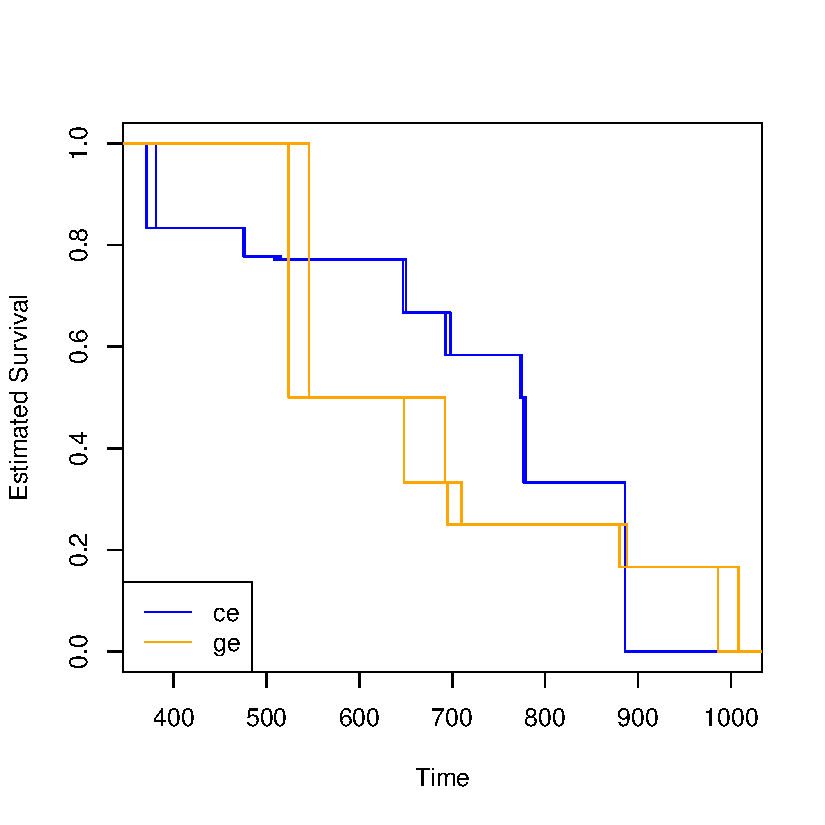
\includegraphics{icenReg-006}


Looking at the plots, we can see a unique feature about the NPMLE for interval censored data. That is, there are \emph{two} lines used to represent the survival curve. This is because with interval censored data, the NPMLE is not always unique; any curve that lies between the two lines has the same likelihood. For example, any curve that lies between the two blues lines maximizes the likelihood associated with \texttt{"ge"} group of mice. 

%Formal statistical tests using the NPMLE are not currently supported by {\bf icenReg}. We recommend using the {\bf interval} package for this. 

\subsection{Semi-parametric models}

Semi-parametric models can be fit with \texttt{ic\_sp} function. This function follows standard regression syntax. As an example, we will fit the \texttt{IR\_diabetes} dataset, which contains data on time from diabetes to diabetic nephropathy. In this dataset, we have the left and right sides of the observation interval containing the true response time and the gender of the patient. 
  
\begin{Schunk}
\begin{Sinput}
> data("IR_diabetes")
> head(IR_diabetes, 3)
\end{Sinput}
\begin{Soutput}
  left right gender
1   24    27   male
2   22    22 female
3   37    39   male
\end{Soutput}
\end{Schunk}
  
We fit the model below. Note that this may be time consuming, as the semi-parametric model is somewhat computationally intense and we are taking \texttt{bs\_samples} bootstrap samples of the estimator. 
  
\begin{Schunk}
\begin{Sinput}
>   fit_ph <- ic_sp(cbind(left, right) ~ gender, model = 'ph', 
+                   bs_samples = 100, data = IR_diabetes)
>   fit_po <- ic_sp(cbind(left, right) ~ gender, model = 'po',
+                   bs_samples = 100, data = IR_diabetes)
\end{Sinput}
\end{Schunk}

The first model by default fits a Cox-PH model, while the second fits a proportional odds model, as controlled by the \texttt{model} argument. We can look at the results using either the \texttt{summary} function, or just directly looking at the results (what is displayed is the same). 
  
\begin{Schunk}
\begin{Sinput}
>   fit_po
\end{Sinput}
\begin{Soutput}
Model:  Proportional Odds
Baseline:  semi-parametric 
Call: ic_sp(formula = cbind(left, right) ~ gender, data = IR_diabetes, 
    model = "po", bs_samples = 100)

           Estimate Exp(Est) Std.Error z-value        p
gendermale   0.4013    1.494    0.1339   2.997 0.002727

final llk =  -1962.4 
Iterations =  25 
Bootstrap Samples =  100 
\end{Soutput}
\begin{Sinput}
>   fit_ph
\end{Sinput}
\begin{Soutput}
Model:  Cox PH
Baseline:  semi-parametric 
Call: ic_sp(formula = cbind(left, right) ~ gender, data = IR_diabetes, 
    model = "ph", bs_samples = 100)

           Estimate Exp(Est) Std.Error z-value       p
gendermale  -0.1402   0.8692   0.07771  -1.805 0.07114

final llk =  -1964.96 
Iterations =  38 
Bootstrap Samples =  100 
\end{Soutput}
\end{Schunk}

For the semi-parametric models, bootstrap samples are used for inference on the regression parameters. The reason for this is that as far as we know, the limiting distribution of the baseline distribution is currently not characterized. In fact, to our knowledge, even using the bootstrap error estimates for the baseline distribution is not valid. Because the regression parameters cannot be seperated in the likelihood function, using the negative inverse of the Hessian for the regression standard errors is not generally valid. However, it has been shown that using the bootstrap for inference \emph{on the regression parameters} leads to valid inference. 

We can use these fits to create plots as well. The \texttt{plot} function will plot the estimated survival curves or CDF for subjects with the set of covariates provided in the \texttt{newdata} argument. If \texttt{newdata} is left equal to \texttt{NULL}, the baseline survival function will be plotted. 
  
Below is a demonstration of how to plot the semi-parametric fit for males and females.
  
\begin{Schunk}
\begin{Sinput}
>   newdata <- data.frame(gender = c('male', 'female') )
>   rownames(newdata) <- c('males', 'females')
>   plot(fit_po, newdata)
\end{Sinput}
\end{Schunk}
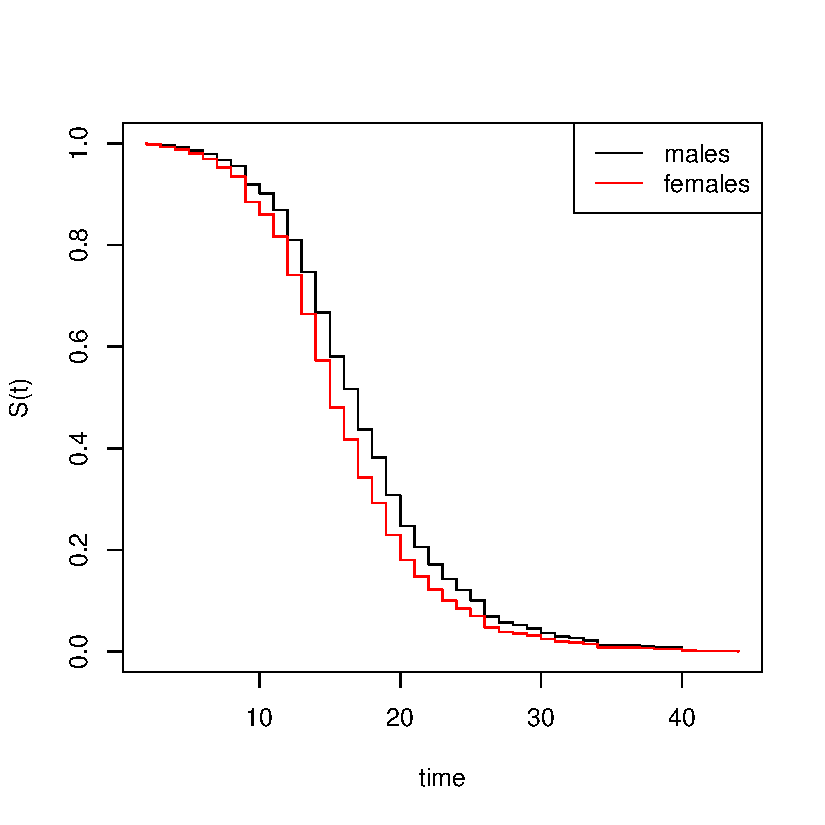
\includegraphics{icenReg-010}

\subsection{Parametric Models}
  
We can fit parametric models in {\bf icenReg} using the \texttt{ic\_par} function. The syntax is essentially the same as above, except that the user needs to specify \texttt{dist}, the parametric family that the baseline distribution belongs to. The current choices are \texttt{"exponential", "weibull"} (default), \texttt{"gamma", "lnorm"} (log-normal), \texttt{"loglogistic"} and \texttt{"generalgamma"} (generalized gamma distribution). The user must also select \texttt{model = "ph"},  \texttt{"po"}, or \texttt{"aft"} as the model type. 
  
It is not necessary to specify \texttt{bs\_samples} for parametric models, as inference is done using the asymptotic normality of the estimators. Fitting a parametric model is typically faster than the semi-parametric model, even if no bootstrap samples are taken for the semi-parametric model. This is because the fully-parametric model is of lower dimensional space without constraints. 
  
Suppose we wanted to fit a proportional odds model to the \texttt{IR\_diabets} data with a baseline gamma distribution. This could be fit by
  
\begin{Schunk}
\begin{Sinput}
> fit_po_gamma <- ic_par(cbind(left, right) ~ gender,
+     data = IR_diabetes, model = "po", dist = "gamma")
\end{Sinput}
\end{Schunk}

  We can examine the regression coefficients in the same way as with the semi-parametric model.
  

\begin{Schunk}
\begin{Sinput}
> fit_po_gamma
\end{Sinput}
\begin{Soutput}
Model:  Proportional Odds
Baseline:  gamma 
Call: ic_par(formula = cbind(left, right) ~ gender, data = IR_diabetes, 
    model = "po", dist = "gamma")

           Estimate Exp(Est) Std.Error z-value        p
log_shape    1.9980    7.377   0.05450  36.670 0.000000
log_scale    0.8248    2.281   0.05563  14.830 0.000000
gendermale   0.3496    1.419   0.13540   2.582 0.009824

final llk =  -2006.619 
Iterations =  4 
\end{Soutput}
\end{Schunk}

  We can also examine the survival/cdf plots in the same way. 
  
\begin{Schunk}
\begin{Sinput}
> plot(fit_po_gamma, newdata, lgdLocation = "topright")
\end{Sinput}
\end{Schunk}
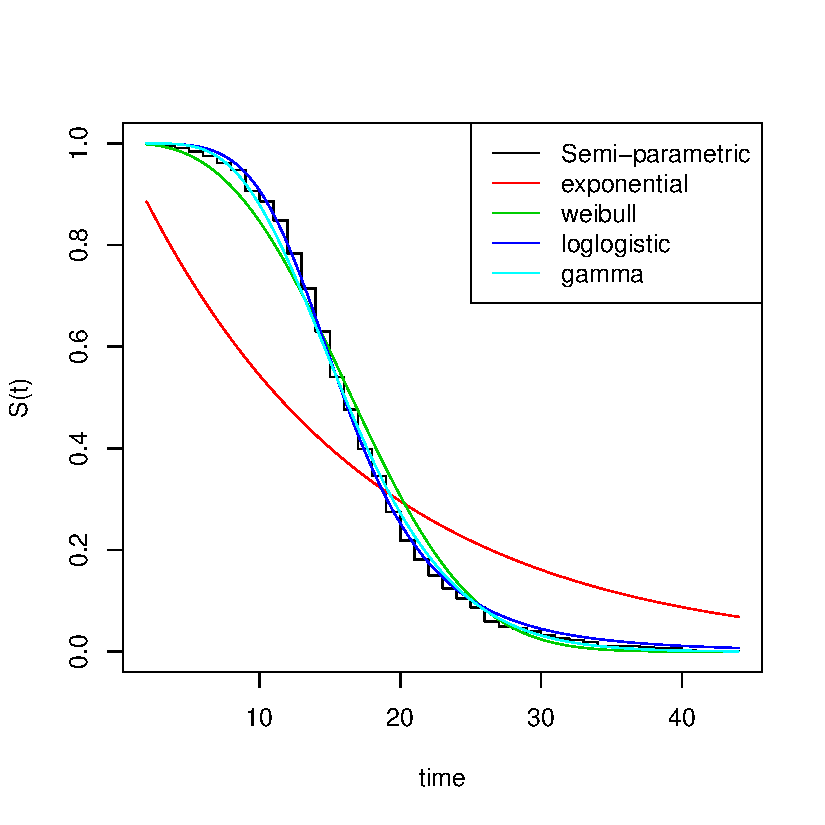
\includegraphics{icenReg-013}

  \subsection{Bayesian Parametric Models}
  
  The option for parametric Bayesian models is also permitted in {\bf icenReg} with the \texttt{ic\_bayes} function. If a flat prior is desired, the use is exactly identical to \texttt{ic\_par}. 
  
\begin{Schunk}
\begin{Sinput}
> flatPrior_fit <- ic_bayes(cbind(left, right) ~ gender,
+     data = IR_diabetes, model = "po", dist = "gamma")
\end{Sinput}
\end{Schunk}

The standard methods work in the same manner as other {\bf icenReg} fits, although the basic output looks fairly different.

\begin{Schunk}
\begin{Sinput}
> flatPrior_fit
\end{Sinput}
\begin{Soutput}
Model:  Bayesian Proportional Odds
Baseline:  gamma 
Call: ic_bayes(formula = cbind(left, right) ~ gender, data = IR_diabetes, 
    model = "po", dist = "gamma")


Iterations = 2001:6996
Thinning interval = 5 
Number of chains = 4 
Sample size per chain = 1000 

1. Empirical mean and standard deviation for each variable,
   plus standard error of the mean:

             Mean      SD  Naive SE Time-series SE
log_shape  1.9965 0.05423 0.0008574       0.001298
log_scale  0.8265 0.05531 0.0008745       0.001481
gendermale 0.3496 0.13281 0.0020999       0.003238

2. Quantiles for each variable:

              2.5%    25%    50%    75%  97.5%
log_shape  1.88941 1.9599 1.9962 2.0333 2.1013
log_scale  0.71752 0.7895 0.8268 0.8633 0.9345
gendermale 0.09344 0.2578 0.3487 0.4386 0.6106

3. MAP estimates:
 log_shape  log_scale gendermale 
    1.9510     0.8671     0.4146 
\end{Soutput}
\end{Schunk}

User that want access to the raw samples can do so through the \texttt{\$samples}
field. 

\begin{Schunk}
\begin{Sinput}
> head(flatPrior_fit$samples)  
\end{Sinput}
\begin{Soutput}
     log_shape log_scale gendermale
[1,]  1.950703 0.8671222  0.4146051
[2,]  2.102873 0.7201840  0.2975855
[3,]  2.027875 0.8094997  0.2271460
[4,]  1.941492 0.9124983  0.3605535
[5,]  1.966307 0.8857313  0.4232492
[6,]  1.987798 0.8446502  0.4705596
\end{Soutput}
\end{Schunk}

This object is a matrix of samples from all chains combined. Alternatively, 
one can look at the samples from each chain individually through the 
\texttt{\$mcmcList} field, with each element corresponding to a given chain. 
Note that \texttt{\$mcmcList} is a \texttt{coda} object of class \texttt{mcmc.list}.

\begin{Schunk}
\begin{Sinput}
> # Accessing the first few samples of the first chain
> head(flatPrior_fit$mcmcList[[1]])
\end{Sinput}
\begin{Soutput}
Markov Chain Monte Carlo (MCMC) output:
Start = 2001 
End = 2031 
Thinning interval = 5 
     log_shape log_scale gendermale
[1,]  1.950703 0.8671222  0.4146051
[2,]  2.102873 0.7201840  0.2975855
[3,]  2.027875 0.8094997  0.2271460
[4,]  1.941492 0.9124983  0.3605535
[5,]  1.966307 0.8857313  0.4232492
[6,]  1.987798 0.8446502  0.4705596
[7,]  1.990583 0.8181635  0.4849160
\end{Soutput}
\begin{Sinput}
> # Accessing the first few samples of the second chain
> head(flatPrior_fit$mcmcList[[2]])
\end{Sinput}
\begin{Soutput}
Markov Chain Monte Carlo (MCMC) output:
Start = 2001 
End = 2031 
Thinning interval = 5 
     log_shape log_scale gendermale
[1,]  1.962868 0.8654202  0.3031021
[2,]  1.897516 0.9227807  0.3506343
[3,]  2.040000 0.8053400  0.6529944
[4,]  2.003793 0.8313133  0.3979533
[5,]  1.992396 0.8275864  0.4201433
[6,]  1.981877 0.8462792  0.3472153
[7,]  1.991957 0.8422614  0.4007510
\end{Soutput}
\end{Schunk}

The log posterior density at each iteration can be accessed through the \texttt{\$logPosteriorDensities} field. Note that this is a list, with each item of the list being a vector from each chain.

\begin{Schunk}
\begin{Sinput}
> head(flatPrior_fit$logPosteriorDensities[[1]])  
\end{Sinput}
\begin{Soutput}
[1] -2007.202 -2008.666 -2007.693 -2009.539 -2009.082 -2007.289
\end{Soutput}
\end{Schunk}


Plotting calls are as standard. Important note: the solids plots the posterior median estimates of the survival curve for a subject with given covariates, \emph{not} the posterior mean estimates!

\begin{Schunk}
\begin{Sinput}
>   plot(flatPrior_fit, newdata,
+        main = 'Posterior Median Estimates')
\end{Sinput}
\end{Schunk}
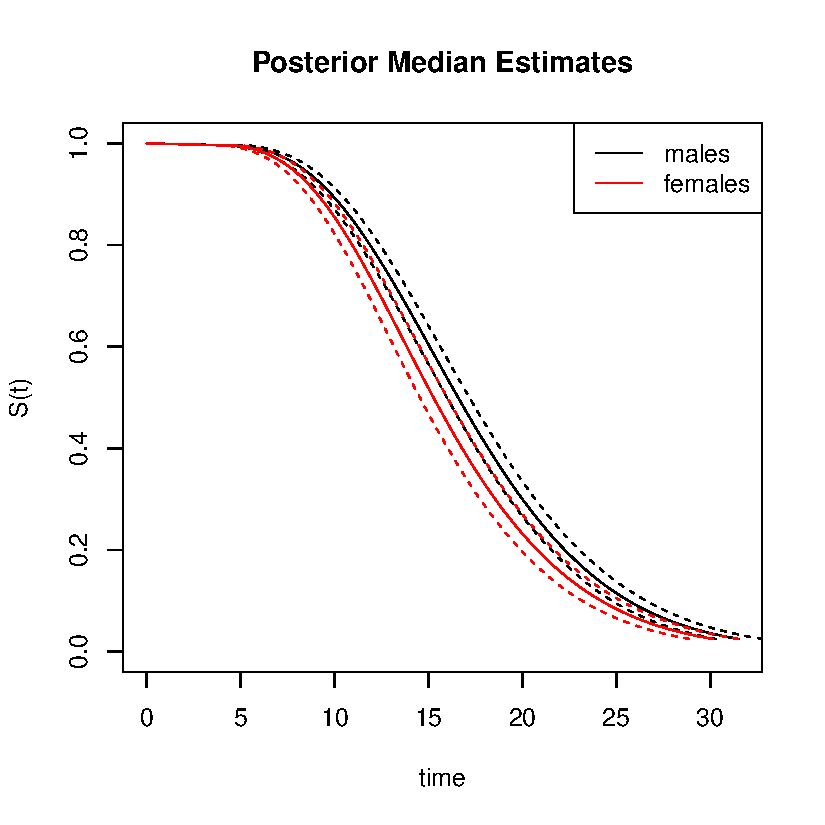
\includegraphics{icenReg-019}


MCMC diagnositic plots can be generated by accessing the \texttt{\$mcmcList} field. 

\begin{Schunk}
\begin{Sinput}
>   plot(flatPrior_fit$mcmcList)
\end{Sinput}
\end{Schunk}
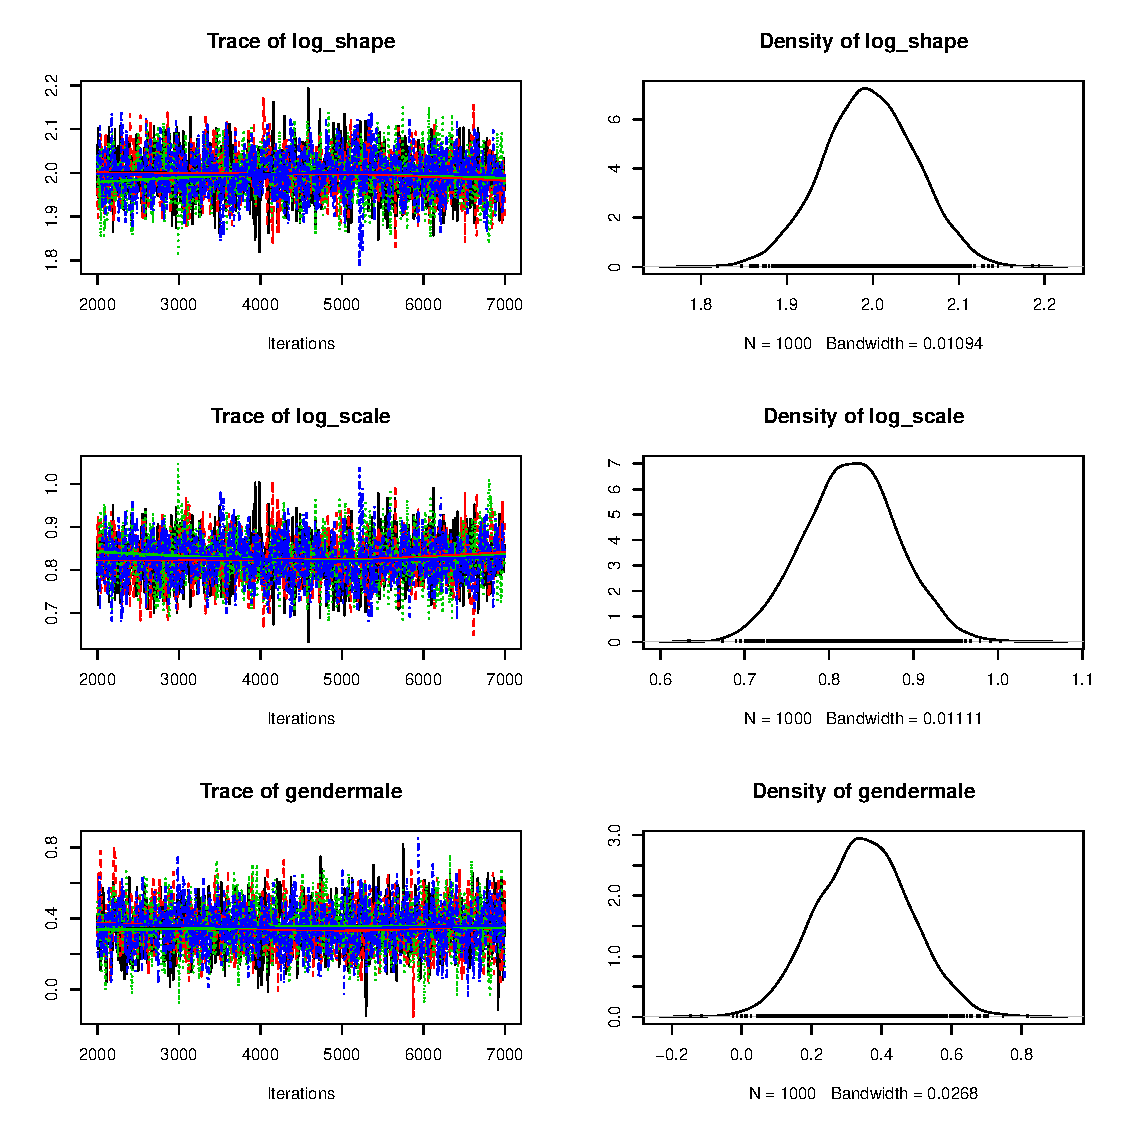
\includegraphics{icenReg-020}

As noted earlier, default behavior is to use a flat prior. If a user wants to use an informative prior, they can provide whichever custom written prior they choose. This function must take in a vector of values corresponding to all the parameters of the model (i.e. first baseline parameters and then regression parameters) and return the log-prior, calculated up to a additive constant. 

This is illustrated with an example where we decide to put a tight prior about the shape parameter (i.e. first baseline parameter) and the regression parameter, and a diffuse prior about the scale parameter. 

\begin{Schunk}
\begin{Sinput}
>  logPriorFunction <- function(x){
+    ans <- 0 
+    ans <- ans + dnorm(x[1], sd = 0.1, log = T)
+    # Tight prior about 1st parameter, log_shape
+    ans <- ans + dnorm(x[2], sd = 10, log = T)
+    # Diffuse prior about 2nd parameter, log_scale
+    ans <- ans + dnorm(x[3], sd = 0.1, log = T)
+    # Tight prior about 3rd parameter, regression parameter
+    return(ans)
+  }    
> informPrior_fit <- ic_bayes(cbind(left, right) ~ gender,
+     data = IR_diabetes, model = "po", dist = "gamma",
+     logPriorFxn = logPriorFunction)
> # Fitting model with prior. 
> 
> informPrior_fit
\end{Sinput}
\begin{Soutput}
Model:  Bayesian Proportional Odds
Baseline:  gamma 
Call: ic_bayes(formula = cbind(left, right) ~ gender, data = IR_diabetes, 
    logPriorFxn = logPriorFunction, model = "po", dist = "gamma")


Iterations = 2001:6996
Thinning interval = 5 
Number of chains = 4 
Sample size per chain = 1000 

1. Empirical mean and standard deviation for each variable,
   plus standard error of the mean:

             Mean      SD  Naive SE Time-series SE
log_shape  1.4497 0.05679 0.0008980       0.001495
log_scale  1.3671 0.05827 0.0009214       0.001525
gendermale 0.1007 0.07797 0.0012328       0.001633

2. Quantiles for each variable:

               2.5%     25%    50%    75%  97.5%
log_shape   1.33765 1.41067 1.4497 1.4892 1.5567
log_scale   1.25574 1.32700 1.3659 1.4065 1.4856
gendermale -0.05112 0.04982 0.1009 0.1519 0.2531

3. MAP estimates:
 log_shape  log_scale gendermale 
   1.46500    1.36800    0.04729 
\end{Soutput}
\end{Schunk}

Note that the posterior mean for \texttt{log\_shape} is pulled down significantly. 

Default behavior for \texttt{ic\_bayes} is to use an adaptive MH block updater, started from the MLE (not MAP) estimate to seed the starting point of the chain and starting proposal covariance. The proposal covariance is updated as more samples are taken. This should work well with informative likelihoods and relatively weak priors. On the other hand, it can be quite problematic with weak likelihoods and relatively strong priors. In such cases, a user may prefer to turn off the MLE initialization. This can be done with the \texttt{bayesControl} function. 

\begin{Schunk}
\begin{Sinput}
> weak_data <- IR_diabetes[1:2,]
> weakData_fit <- ic_bayes(cbind(left, right) ~ gender,
+     data = weak_data,
+     model = "po", dist = "gamma",
+     logPriorFxn = logPriorFunction,
+     controls = bayesControls(useMLE_start = F))
> plot(weakData_fit$mcmcList)
\end{Sinput}
\end{Schunk}
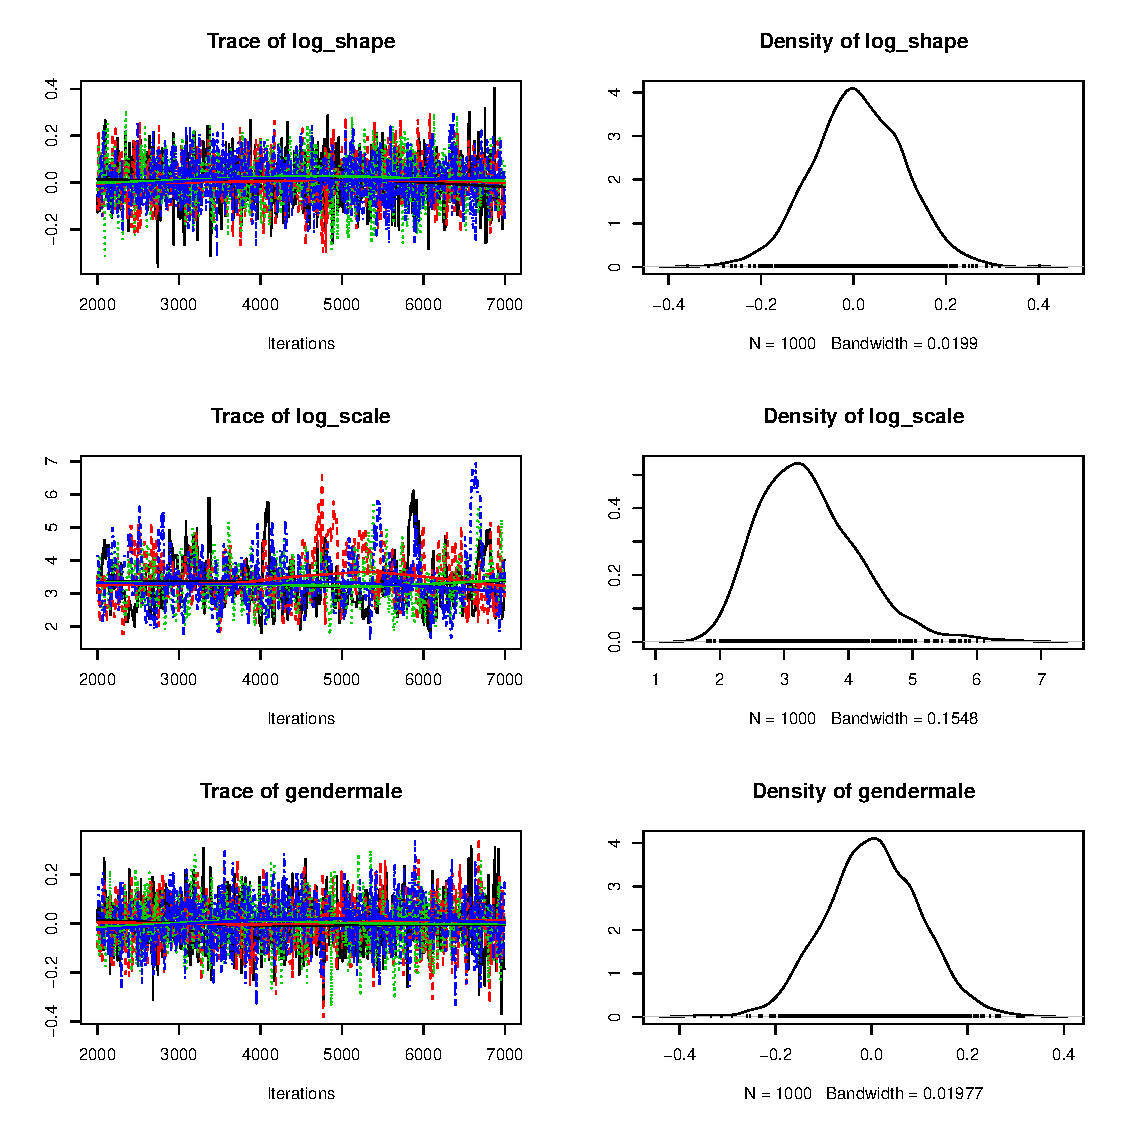
\includegraphics{icenReg-022}

Note that in this sample, we see evidence that the chain has not properly mixed, especially in regards to the \texttt{log\_scale} parameter. Using \texttt{bayesControls}, we could increase both the samples and burnIn to address this issue. 

\subsection{Extracting Estimates and CIs}

We can also extract survival estimates and confidence/credible intervals
for a given set of covariates using the \texttt{survCIs}. 

\begin{Schunk}
\begin{Sinput}
> # Extract estimates for inverse CDF
> invCDF_ests = survCIs(informPrior_fit, newdata, 
+                       p = seq(from = 0.05, to = .95, by = 0.2))
> # Extract estimates for *CDF* probabilities at given values
> CDF_ests = survCIs(informPrior_fit, newdata, 
+                    q = seq(from = 5, to = 25, by = 5))
> invCDF_ests
\end{Sinput}
\begin{Soutput}
Model call:
  ic_bayes(formula = cbind(left, right) ~ gender, data = IR_diabetes, 
    logPriorFxn = logPriorFunction, model = "po", dist = "gamma")
Credible Level = 0.95 
Rowname:  males 
     Percentile estimate (mean) estimate (median)     lower     upper
[1,]       0.05        6.034928          6.036237  5.504032  6.534367
[2,]       0.25       10.933506         10.935934 10.358423 11.486894
[3,]       0.45       14.662174         14.667501 14.042197 15.276086
[4,]       0.65       18.815478         18.820303 18.061075 19.553142
[5,]       0.85       25.122799         25.106139 24.120340 26.173859
Rowname:  females 
     Percentile estimate (mean) estimate (median)     lower     upper
[1,]       0.05        5.852019          5.854968  5.312181  6.371661
[2,]       0.25       10.576260         10.580831  9.943573 11.195182
[3,]       0.45       14.198484         14.204869 13.469342 14.903160
[4,]       0.65       18.275854         18.274579 17.454299 19.094438
[5,]       0.85       24.540428         24.534111 23.479829 25.649572
\end{Soutput}
\begin{Sinput}
> CDF_ests
\end{Sinput}
\begin{Soutput}
Model call:
  ic_bayes(formula = cbind(left, right) ~ gender, data = IR_diabetes, 
    logPriorFxn = logPriorFunction, model = "po", dist = "gamma")
Credible Level = 0.95 
Rowname:  males 
     Time estimate (mean) estimate (median)      lower      upper
[1,]    5      0.02773927        0.02742149 0.01982986 0.03771561
[2,]   10      0.20308927        0.20278403 0.17698341 0.23161636
[3,]   15      0.46788548        0.46752416 0.43583591 0.50143756
[4,]   20      0.69755647        0.69745734 0.66761488 0.72767791
[5,]   25      0.84723250        0.84761978 0.82389244 0.86927823
Rowname:  females 
     Time estimate (mean) estimate (median)      lower      upper
[1,]    5      0.03059472        0.03022538 0.02165862 0.04174449
[2,]   10      0.21990287        0.21942076 0.18966032 0.25308781
[3,]   15      0.49298199        0.49263737 0.45502311 0.53249776
[4,]   20      0.71827709        0.71821950 0.68573509 0.74959068
[5,]   25      0.85973115        0.85997744 0.83580071 0.88171151
\end{Soutput}
\end{Schunk}

Note that the output from survCIs is what is used to create the 
plots for \texttt{icenReg} fits, so if one wanted to export the plotting to 
\texttt{ggplot} or plot the posterior mean rather than the posterior median, for example, one could do so directly with \texttt{survCIs}. 

\section{Inspecting model fit}

\subsection{Examining Baseline Distribution}
  
Althought the semi-parametric model is more flexible, and thus more robust to unusual baseline distributions, there are many reasons one may decide to use a parametric model instead. One reasons is that, as stated earlier, we are not aware of any general distributional theory regarding the baseline distribution, outside of the univariate case with case I interval censored data. Even in this case, the estimator is highly inefficient, observing convergence rates of $n^{1/3}$ instead of the more standard $n^{1/2}$. Because of this, making inference about values that directly require the baseline distribution, such as creating a confindence interval for the median for subjects with a given set of covariates, cannot be done with the semi-parametric model. 
  
  %Secondly, we have found that
  %when it comes to cross-validation (to be described shortly), 
  %we often found the semi-parametric estimator
  %to be overly optimistic for some loss functions in comparison with a parametric model. 
  
However, even if a parametric model is used for final inference, the semi-parametric model is still useful for assessing model fit. This is especially important for interval censored data, as we do not have the option of examining typical residuals or histograms as we would if the outcome was uncensored. {\bf icenReg} has the function \texttt{diag\_baseline} that plots several choices of parametric baseline distributions against the semi-parametric estimate. If the parametric distribution shows no systematic deviations from the semi-parametric fit, this implies the choice of parametric family may do a reason job of describing the underlying distribution. If there are clear deviations, this model should not be trusted. 
  
To use \texttt{diag\_baseline}, you must provide either a fitted model, or a formula, data and model. You then select the parametric families that you would like plotted against the non-parametric estimate (default is to fit all available). As an example, suppose we wanted to examine the different parametric fits for the \texttt{IR\_diabetes} dataset. This could be done with 
  
\begin{Schunk}
\begin{Sinput}
> diag_baseline(cbind(left, right) ~ gender,
+     model = "po",
+     data = IR_diabetes,
+     dists = c("exponential", "weibull", 
+               "loglogistic", "gamma"),
+     lgdLocation = "topright")
\end{Sinput}
\end{Schunk}
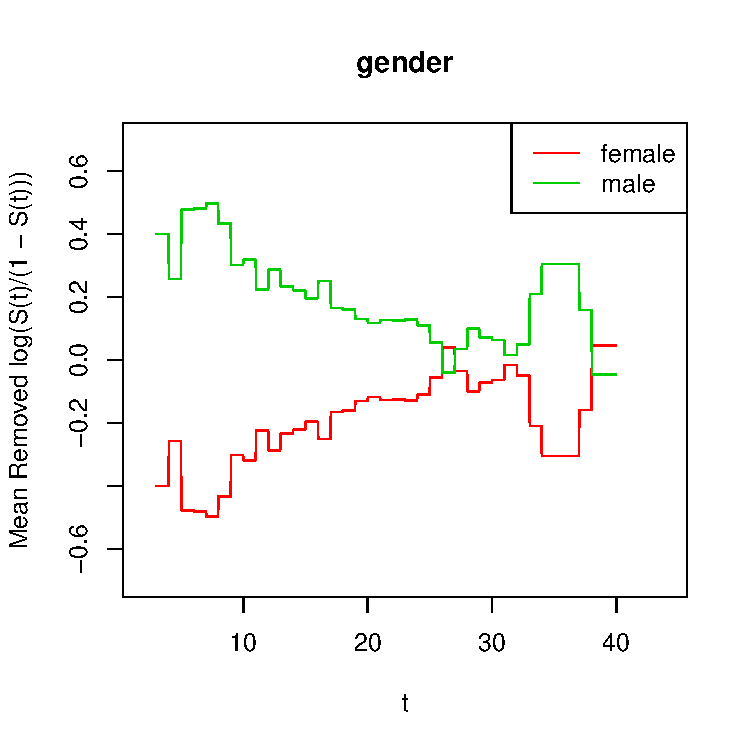
\includegraphics{icenReg-024}

Alternatively, using the fits from earlier, we can just call
  
\begin{Schunk}
\begin{Sinput}
> diag_baseline(fit_po, lgdLocation = "topright",
+               dists = c("exponential", "weibull", 
+                         "loglogistic", "gamma")
+               )
\end{Sinput}
\end{Schunk}

Visual diagnostics are always subjective, but in this case we definitively know that the exponential fit is not appropriate and we believe the gamma baseline is most appropriate for the proporitonal odds model (although there is not overwhelming evidence that it is best). 
  
\subsection{Examining Covariate Effect}
  
Although semi-parametric models do not make assumptions about the parametric family of the baseline distribution, both fully-parametric and semi-parametric models make assumptions about the form of the covariate effect, akin to the link function in generalized linear models. 
  
A rule of thumb for identifying gross violations of proportional hazards is to check if the Kaplan Meier curves cross; if they do, and this cross appears not purely by chance, the proportional hazards assumption seems inappropriate. 
  
This can naturally extend to the case of interval censored data by replacing the Kaplan Meier curves with the NPMLE. Also, this informal test can be generalized to the proportional odds model; the proportional odds assumption also implies that survival curves that differ only by a constant factor of the odds of survival should not cross. 
  
Another method of assessing involves transforming yoursurvival estimates such that if the assumptions are met, the difference in transformed survival will be constant. For the proportional hazards model, this is the complementary log-log tranformation (i.e. $\log (-\log(s) )$). For the proportional odds model, this is the logit transformation (i.e. $\log(s/(1-s))$ ).
  
Plotting these functions can be done automatically in {\bf icenReg} using the \texttt{diag\_covar} function. The basic flow is that function takes in the fit, divides the data up on a covariate of interest. If it is categorical, it simply breaks up by category, if it is numeric, it attempts to find break point to evenly split up the data. Then, for each subset of the data, it fits the corresponding semi-parametric model and plots the transformation of the baseline distribution. 
 
To demonstrate, suppose we wanted to assess whether the Cox-PH or proportional odds model was more appropriate for the \texttt{IR\_diabetes}. This could be done by 
 
\begin{Schunk}
\begin{Sinput}
> diag_covar(fit_po, lgdLocation = "topright", 
+            main = "Checking Proportional Odds")
> diag_covar(fit_ph, lgdLocation = "topright", 
+            main = "Checking Proportional Hazards")
\end{Sinput}
\end{Schunk}

We see that especially for gender, the porportional odds
seems somewhat more appropriate (the difference between 
transformed values seems more constant). This agrees
with the fact that the likelihood is approximately 2.5 greater
for the proportional odds model than Cox-PH. 
  
\begin{minipage}[t]{.85\linewidth}%
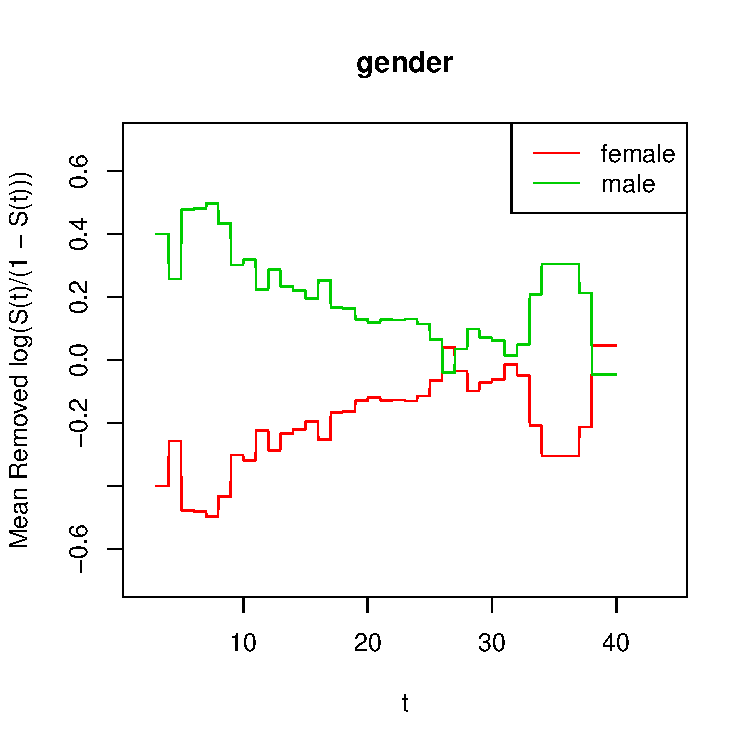
\includegraphics{icenReg-027}
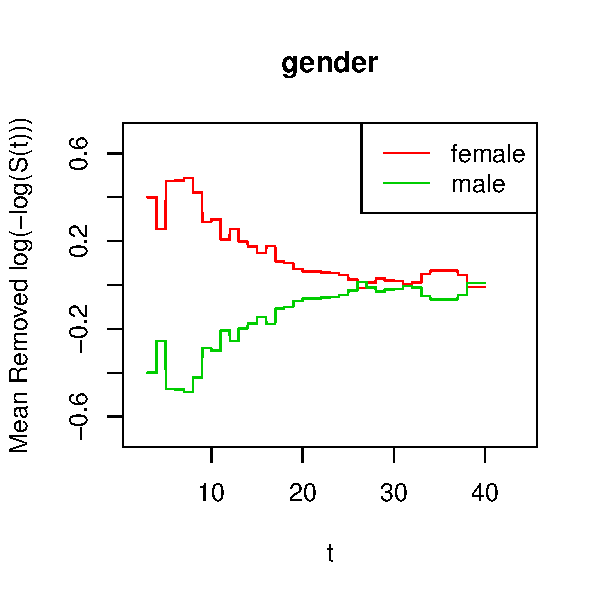
\includegraphics{icenReg-028}
\end{minipage}

%\subsection{Imputed Cross Validation}

%  Cross validation is a popular method for evaluating how well a model will perform 
%  on new data. In general, 
%  the idea is simple enough: to get an estimate of some loss function on
%  out of sample data for a given model, we split the data into training
%  and validation datasets. The training dataset is used to fit the model
%  (without touching the validation data). Then an estimate of the out of
%  sample error can be generated by predicting the response in the validation
%  dataset and directly computing the loss function. In K-fold cross validation,
%  K disjoint subsets of the data are used as validation datasets and the process
%  is repeated K-times. 
  
%  For censored data, this generic recipe is not so simple. In particular, if 
%  a value in the validation set is censored, there is typically no direct
%  method for calculating the contribution to the loss function 
%  associated with this observation. 
  
%  One method to deal with censoring that has appeared in the literature is to calculate
%  likelihood over the validation data set. As an alternative, we offer an imputation
%  based approach. To calculate the
%  average loss function, we take several imputations (or samples) of the 
%  interval censored data condtional on the covariates \emph{and censoring interval}
%  (i.e. the distribution is truncated such that the imputation will fall inside the
%  given censoring interval). The average loss across all imputations is then taken
%  as the evaluated loss. 
  
%  To impute the data, we first take a sample of the posterior parameters and conditional
%  on the parameters and censoring interval, we sample the censored values. An important
%  note is that {\bf icenReg} does \emph{not} sample the baseline parameters, but only
%  the regression parameters for the semi-parametric model. This means that the 
%  uncertainity in the baseline parameteris is ignored. 
%  For the fully parametric model, both the regression and
%  baseline parameters are sampled.

%  For the prediction, the median value conditional on the parameter estimates is used. 
%  This is \emph{not} neccesarily the estimate that minimizes the loss function, but it 
%  is generally a reasonable estimate. 
  
%  Cross validation can be done with {\bf icenReg}'s \texttt{icenReg\_cv} function. 
%  This takes a regression model (either from \texttt{ic\_par} or \texttt{ic\_sp}), and a
%  loss function to be calculated.
%  CAUTION: When using cross-validation on an \texttt{ic\_sp} fit, the total number of 
%  models fit will be \texttt{fold} (default = 10) x \texttt{bs\_samples}. This can get
%  very expensive very quickly!
  
%  The default loss function is \texttt{abs\_inv}, which is 
%  defined as 
  
%  \begin{verbatim}
%  abs_inv <- function(pred, t_val) {
%    mean(abs(1/(pred + 1) - 1/(t_val + 1)))
%  }
%  \end{verbatim}

%  Although we believe this to be a reasonable loss function for survival data
%  (heavy penalizes for missing subjects that are at high risk, does not heavily 
%  penalizing for not being precise with low-risk subjects as long as they are identified as low risk),
%  this function is not the final say in loss functions. 
%  A user can write their own loss function, which should take in arguments
%  \texttt{pred} and \texttt{t\_val}, where \texttt{pred} is the predicted
%  value and \texttt{t\_val} is the true response value. 
  
%  Imputed cross validation can then be used as such:
  
%  \begin{verbatim}
%  icenReg_cv(fit = fit_po, loss_fun = abs_inv)
%  \end{verbatim}
  
  
  \section{Appendix}
  
  \subsection{Parallel Bootstrapping}
  
%  Both the bootstrap and cross validation statistics can be extremely computationally
%  expensive, yet also are both embarrassingly parallel problems. As such, they are 
%  written take advantage of multiple cores via the {\bf doParallel} package. 
%  Below is demonstrated how to run the bootstrap and cross validation using 
%  four cores. 
 
Bootstrapping can be very computationally intensive. Fortunately, it is also embarrassingly parallel. As such, icenReg is written to work seamlessly with \texttt{doParallel}
  
\begin{verbatim}
> library(doParallel)
> myCluster <- makeCluster(4)  #uses 4 cores
> registerDoParallel(myCluster)
> fit <- ic_sp(cbind(left, right) ~ gender,
+            data = IR_diabetes, model = "po",
+            bs_samples = 50, useMCores = TRUE)
>stopCluster(myCluster)
\end{verbatim}
  
  
\end{document}
